\chapter{CMS DETECTOR}
\label{chap:Detector}

The Compact Muon Solenoid (CMS) detector is a multi-purpose detector designed to accurately measure the energy and momentum of all particles produced in proton-proton or heavy ion collisions. Figure~\ref{fig:CMS} shows a schematic of the detector as a whole. The CMS detector is 21.6 m long, 14.6 m in diameter, and weighs 12500 t. 
Moving radially outward from the interaction point, the sub-detectors are the silicon pixel and strip tracker (Section~\ref{sec:Tracker}), the electromagnetic calorimeter (Section~\ref{sec:ECAL}), the hadron calorimeter (Section~\ref{sec:HCAL}), and the muon system (Section~\ref{sec:Muon}). For a full description of the CMS detector, see Reference~\cite{Chatrchyan2008zzk}. 

\begin{figure}[h!]
	\centering
	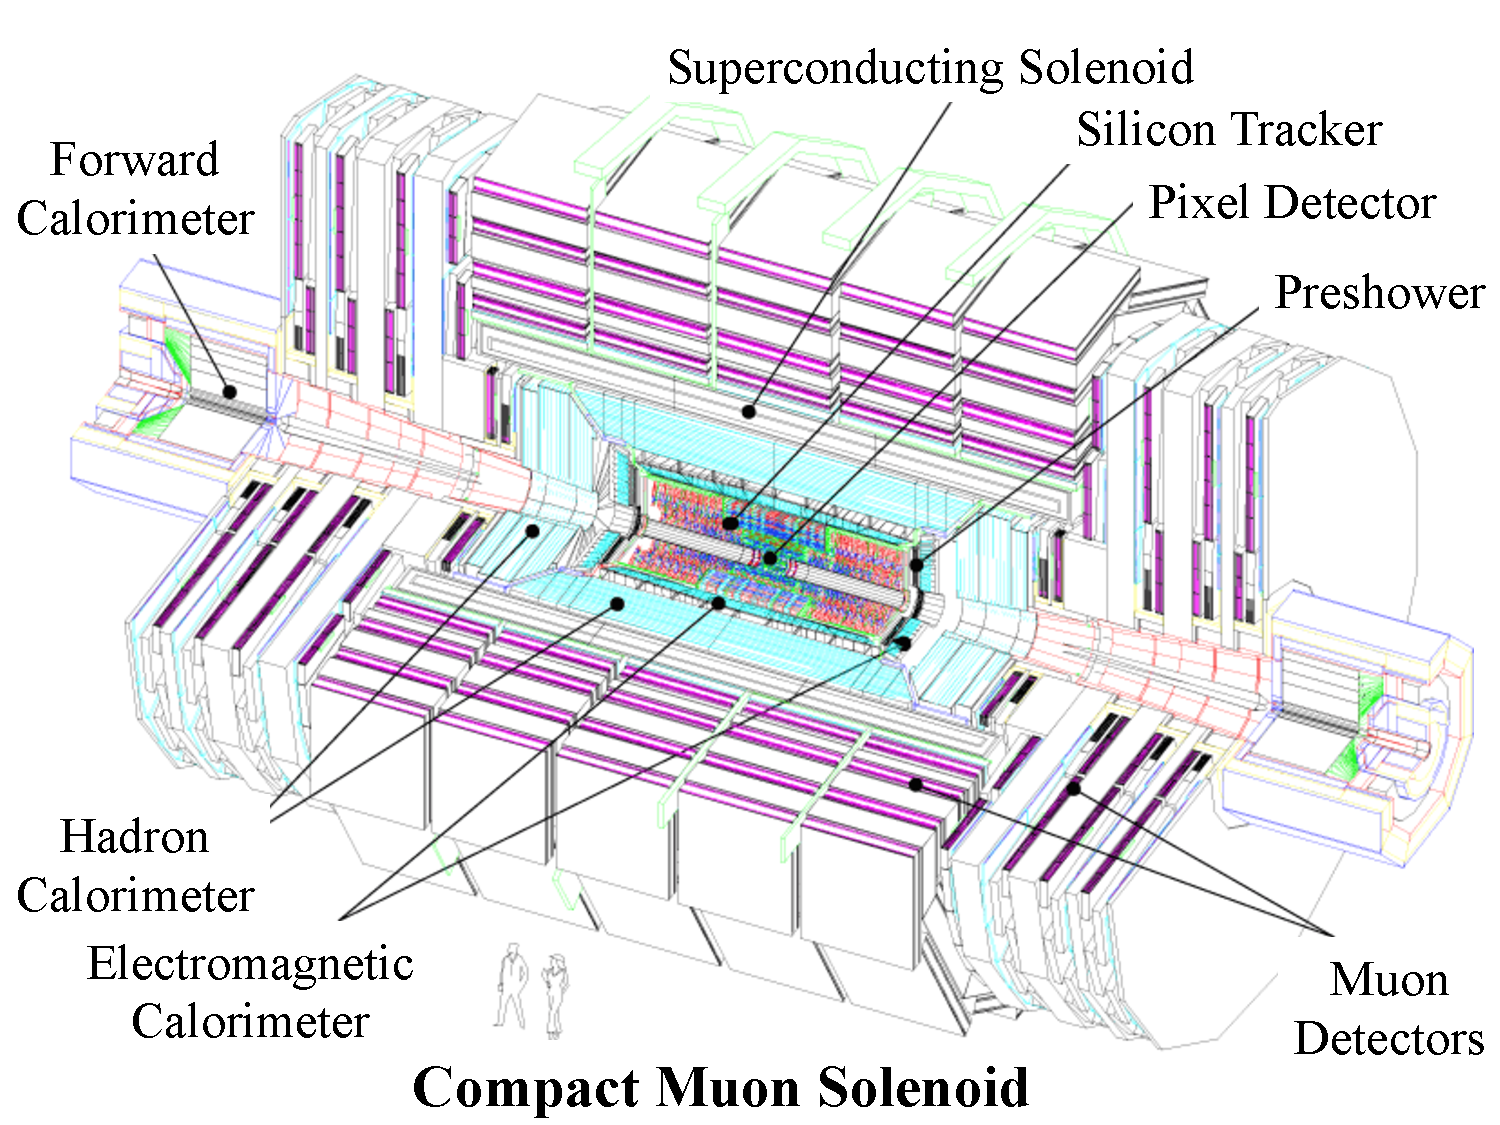
\includegraphics[width=0.8\textwidth]{Figures/Detector/cms_labelled.pdf}
       \caption{Schematic of the CMS detector.
	}
   	\label{fig:CMS}
\end{figure}

%%%%%%%%%%%%%%%%%%%%%%%%%%%%

\section{Coordinate system}
\label{sec:coordinates}
The origin of the CMS detector coordinate system is located at the nominal collision point. The $z$-axis is oriented along the beam direction, with the positive $z$-axis pointing in the counter-clockwise direction when viewing the LHC from above. The $y$-axis points vertically upward, and the $x$-axis points toward the center of the LHC. The $xy$-plane is referred to as the transverse plane.

Due to the nature of particle collisions, however, Cartesian coordinates are often not the most convenient. Because protons are not elementary particles, it is actually the individual quarks or gluons within the proton that interact during the collision. This means that the collision will not be at rest in the lab frame, but will have some non-zero velocity along the $z$-axis. To deal with this, it is beneficial to use coordinates that are invariant under boosts in the $z$-direction. CMS follows the particle physics convention of describing the position of a particle in terms of its transverse momentum, azimuthal angle, and pseudorapidity. The transverse momentum \pt is defined as the magnitude of the momentum in the $xy$-plane. The azimuthal angle $\phi$ is defined in the transverse plane, with $\phi  = 0$ corresponding to the positive $x$-axis. Finally, the pseudorapidity is defined as $\eta = -\ln{\tan{ (\theta / 2 )} } $, where the polar angle $\theta$ is measured from the $z$-axis. Distances between particles are generally expressed using the \dR~variable, where $\dR = \sqrt{\Delta \eta^2 + \Delta \phi^2}$.

%%%%%%%%%%%%%%%%%%%%%%%%%%%%

\section{Superconducting solenoid}
\label{sec:magnet}

One of the most important components of the CMS detector is the superconducting solenoid that provides the bending power necessary to precisely measure the momentum of all charged particles produced in the collision. The solenoid is a 4-layer niobium-titanium coil embedded in aluminum and aluminum alloy. The magnet is located between the calorimeters and the muon system. It is 12.5 m long and has an inner diameter of 6 m. It is capable of producing magnetic fields up to 4 T, although the magnet is generally operated at 3.8 T to prolong its lifetime. At full current, the magnet has a stored energy of 2.6~GJ. A 12,000 ton steel yoke made up of 5 wheels in the barrel and 3 endcap disks serves to return the magnetic flux. The solenoid is suspended in a vacuum cryostat and cooled to 4.5 K with liquid helium. A detailed description of the CMS magnet can be found in Reference~\cite{magnetTDR}. Figure~\ref{fig:magnet} shows the calculated magnetic field in a longitudinal slice of the CMS detector.

\begin{figure*}[h!]
	\centering
	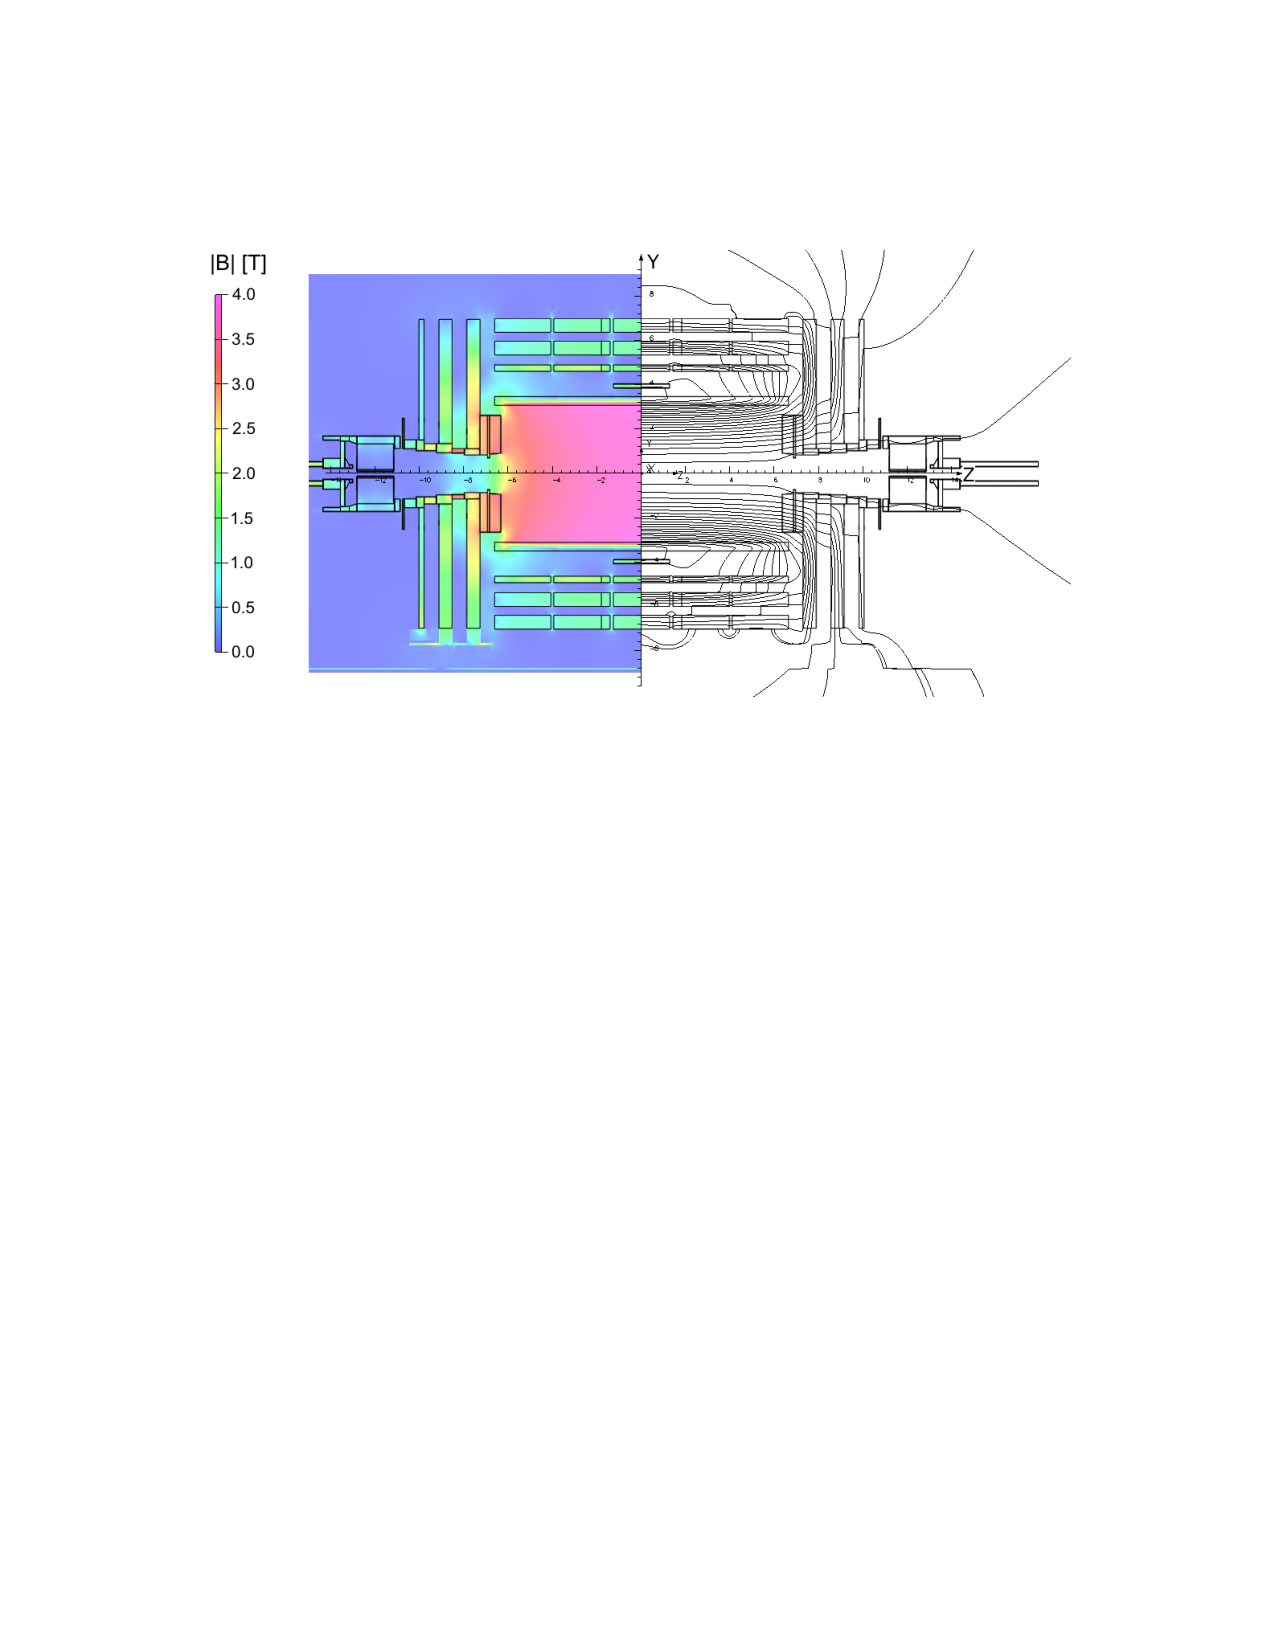
\includegraphics[width=\linewidth]{Figures/Detector/magnet.pdf}
       \caption{Calculated magnetic field $|\vec{B}|$ for a longitudinal slice of the CMS detector when operated at a central magnetic flux density of 3.8 T. In the right-hand portion of the figure, each magnetic field line represents a magnetic flux step of 6 Wb. Reprinted from Reference~\cite{CMSMagnetField}.}
       \label{fig:magnet}
\end{figure*}

%%%%%%%%%%%%%%%%%%%%%%%%%%%%

\section{Tracker}
\label{sec:Tracker}

The innermost sub-detector is the silicon tracker~\cite{trackerTDR,trackerTDRAddendum}. The tracker must provide enough information to accurately reconstruct the trajectories of charged particles to a high level of precision. This is accomplished through the use of silicon semiconductors, which rely on the properties of p-n junctions to detect charged particles. A p-n junction is created by bringing a p-type semiconductor into contact with an n-type semiconductor. For p- and n-type semiconductors, the crystal lattice of the semiconductor is doped to either donate or accept extra electrons, respectively. In a p-n junction, the extra electrons in the n-type semiconductor migrate and combine with the electron holes in the p-type semiconductor. This creates a depletion region in the center of the crystal. Charged particles passing through the depletion region will create electron-hole pairs that move towards either end of the junction when an external electric field is applied. The collected charge is proportional to the energy deposited in the detector.

The overall dimensions of the tracker are 5.6 m in length and 1.2 m in radius. The full tracking system is cylindrical in shape and is comprised of a barrel and two endcaps, each of which is split into layers of silicon pixel detectors and layers of silicon micro-strip detectors. In total, there are 48 million $150\times100~\mu$m pixels and 9.6 million strips that are between 80 and 180 $\mu$m wide. Figure~\ref{fig:TrackerLayout} shows a schematic drawing of the layout of the tracker subsystems. For charged hadrons with \pt less than 20 GeV, the \pt can be measured with a resolution of $1\%$. 

\begin{figure*}[h!]
	\centering
	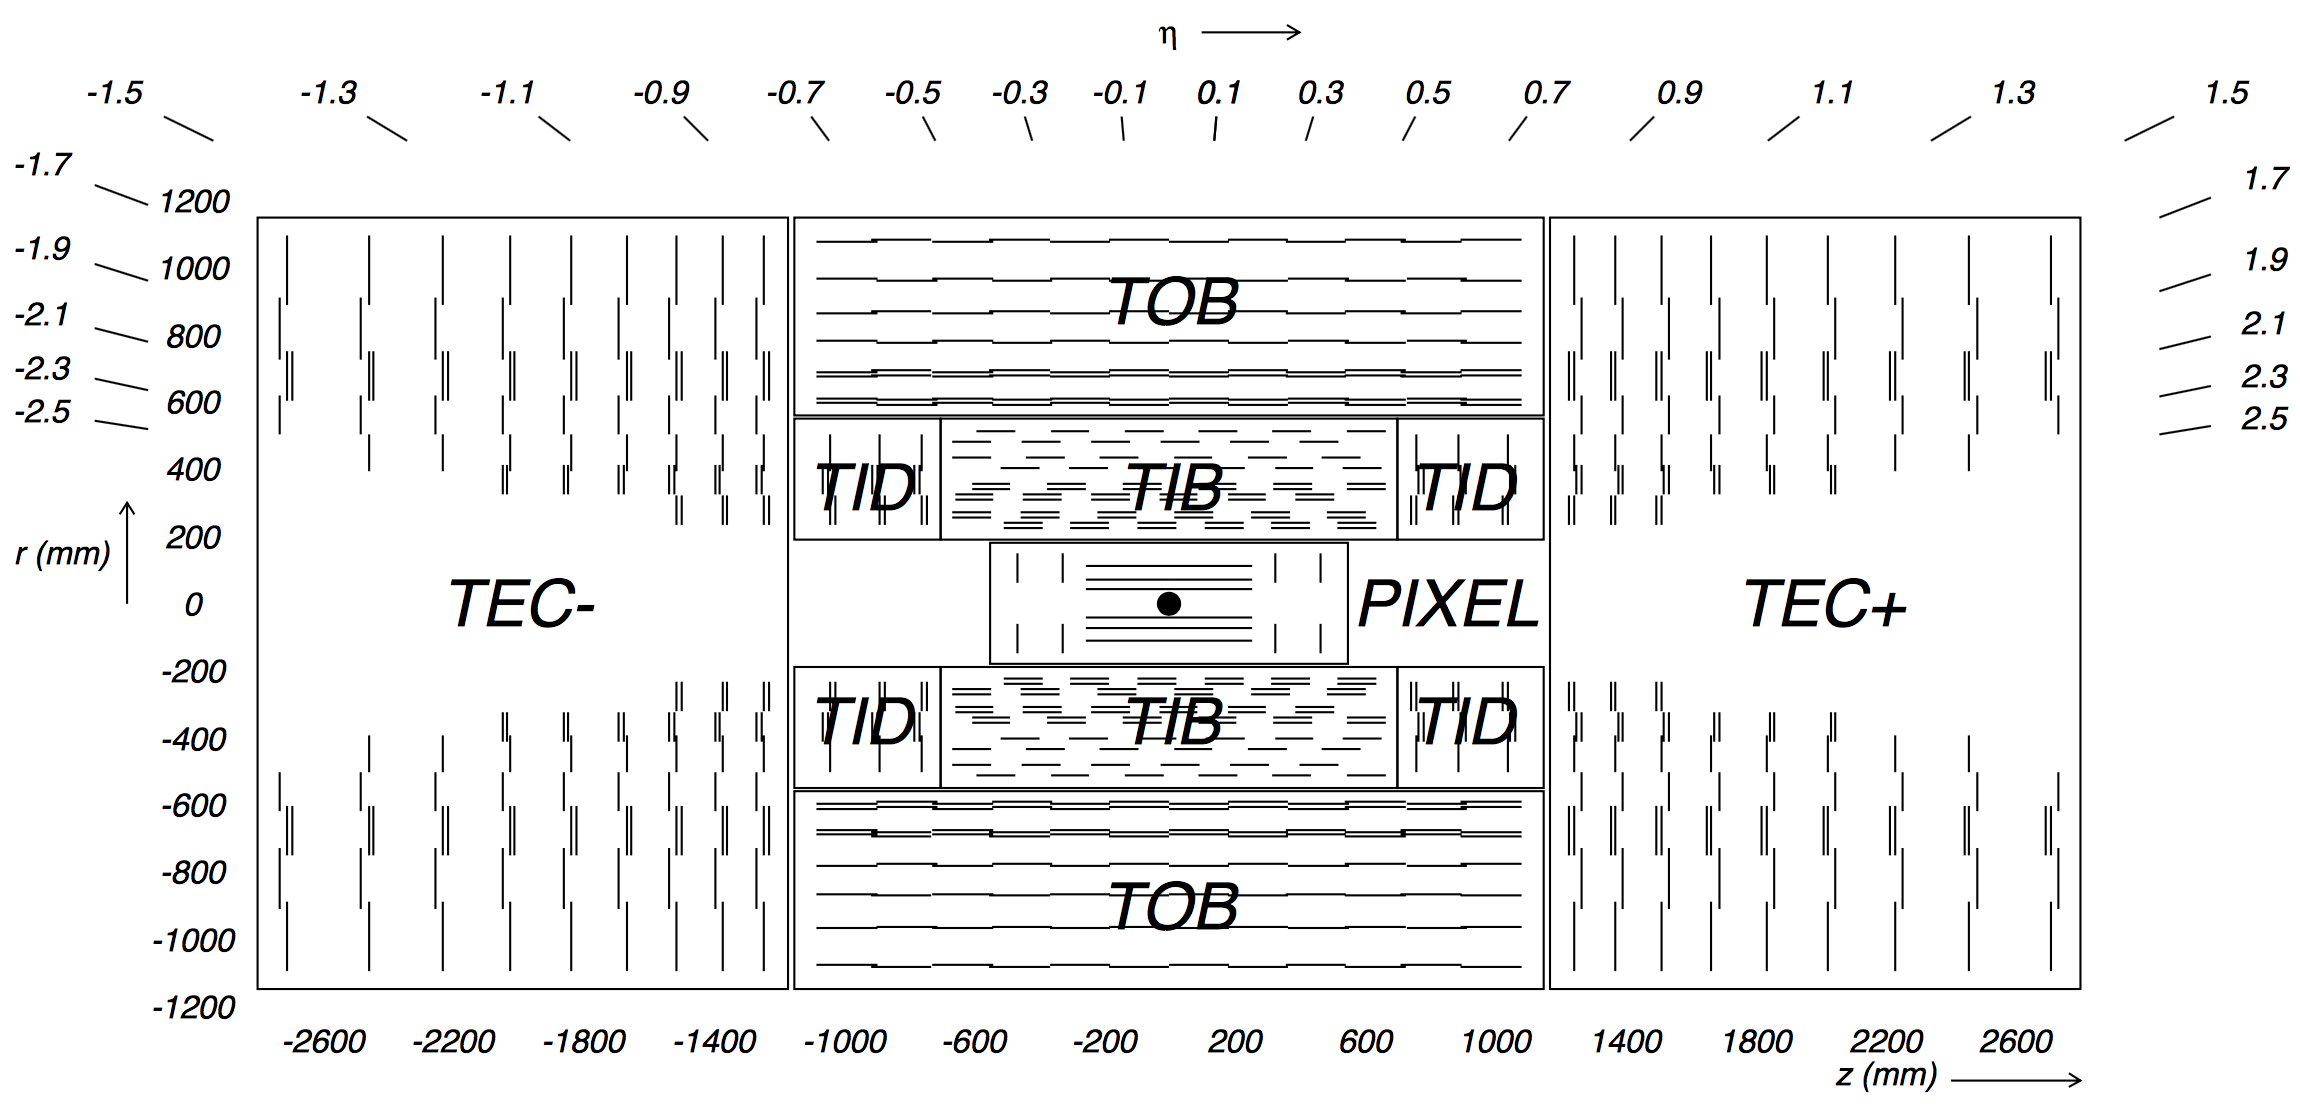
\includegraphics[width=\linewidth]{Figures/Detector/tracker_layout.png}
       \caption{Schematic of the CMS tracker system. Detector modules are represented by single lines, and back-to-back modules are represented by double lines. The strip tracker is further divided into the Tracker Inner/Outer Barrel (TIB/TOB), Tracker Inner Disk (TID) and the Tracker Endcap (TEC). Reprinted from Reference~\cite{Chatrchyan2008zzk}.}
   	\label{fig:TrackerLayout}
\end{figure*}

\subsection{Pixel detectors}
\label{sec:TrackerPixel}

Due to the high occupancy of the tracker within 10 cm of the beam pipe, pixel detectors rather than strip detectors are used as the innermost layers of the tracker. Three layers in the barrel and two disks of pixel detectors in the endcap give three high-precision points for every charged particle moving away from the interaction point. The small pixel size of $150\times100~\mu$m is critical for accurate secondary vertex reconstruction, for forming seed tracks used for high level triggering (see Chapter~\ref{chap:Trigger}), and for the reconstruction of charged particles in the event (see Chapter~\ref{sec:EventReconstruction}). The three barrel layers are 53 cm long and are located at mean radii of 4.4, 7.3 and 10.2 cm. The endcap modules extend radially from 6 to 15 cm and are placed on each side at $z=\pm 34.5$ and $z=\pm 46.5$~cm. The endcaps extend the coverage of the sub-detector to $|\eta|~<~ 2.5$. 
%Yutaro: An interpolation of the signal amplitudes gives a spacial resolution of 15-20 mum, (because charge is shared between several pixels due to the geometry and the magnetic field)

\subsection{Strip detectors}
\label{sec:TrackStrip}
Moving radially beyond the pixel detectors are the silicon strip trackers. These operate on the same basic principles as the pixel detectors, but each silicon strip is 10 cm $\times~80~\mu$m, giving a precise position measurement along one dimension only. In the barrel, the strips run parallel to the $z$-axis with a pitch, or spacing between strips, between 80 and 183 $\mu$m. Strips in the endcaps are aligned radially with a pitch between 100 and 184 $\mu$m. In total there are 10 layers of strip sensors in the barrel and 12 layers in the endcaps.

The tracker has a spatial resolution of 25-50 $\mu$m perpendicular to the strip direction. In order to improve the precision of the detector in the direction parallel to the strips, several of the layers are arranged in pairs. By aligning the second layer 100 mrad off from the strips in the first layer, a spatial resolution of 230 to 530 $\mu$m can be achieved. These back-to-back modules are represented by double lines in Figure~\ref{fig:TrackerLayout}.

%Yutaro: paragraph on the alignment system for the strips.

%%%%%%%%%%%%%%%%%%%%%%%%%%%%

\section{Electromagnetic Calorimeter (ECAL)}
\label{sec:ECAL}

Beyond the tracker is the electromagnetic calorimeter (ECAL), the most important sub-detector for this analysis~\cite{ECAL_TDR,ECAL_TDRAddendum}. The ECAL measures the energies deposited by photons and electrons when they are stopped by the detector. For energies above 10 MeV, electrons lose energy primarily through the production of photons in bremsstrahlung. Photons lose energy through the production of $e^+e^-$ pairs \cite{Calo}. Therefore, when an energetic electron or photon is incident on one of the crystals of the ECAL, the result is an electromagnetic cascade (``shower") of photons and electrons with successively lower energies.

The CMS ECAL is designed to contain the full electromagnetic shower from electrons and photons with initial energies as high as a few TeV. It is a homogeneous calorimeter made with 75,848 scintillating lead tungstate PbWO$_4$ crystals. The ECAL is divided into a barrel region (EB) covering $|\eta| < 1.479$ and two endcap regions (EE) covering $1.479 < |\eta| < 3.0$.  Each region includes a single layer of PbWO$_4$ crystals. In the barrel, the crystals have a truncated pyramidal shape with a radial depth of 23 cm. The front face of the crystal has dimensions 22 $\times$ 22 mm$^2$, and the rear face has dimensions 26 $\times$ 26 mm$^2$. In the endcap, the crystals are 22 cm long and have a cross section of 28.62 $\times$ 28.62 mm$^2$ on the front face and 30.0 $\times$ 30.0 mm$^2$ on the rear face. 

Lead tungstate is an inorganic scintillator. The passage of charged particles produce electron-hole pairs in the conduction and valence bands of the material, and light is emitted when the electrons return to the valence band. There are several properties of PbWO$_4$ that make it an ideal choice for the scintillating material of the CMS ECAL. Its Moli\`{e}re radius, defined as the radius of a cylinder containing 90\% of the shower's energy deposition, is only 2.2 cm, allowing for excellent position resolution and separation between showers. The latter is particularly important when trying to distinguish photons from isolated $\pi^0\rightarrow\gamma\gamma$ decays. The fast response time of lead tungstate is also critical. Approximately 80\% of the light is emitted within 15 ns \cite{Calo}, making it possible for each particle to be assigned to the correct bunch crossing. 

Another positive feature of PbWO$_4$ is that it is dense enough (8.3 g/cm$^3$) that the ECAL can fit into a relatively compact area. The depth of material that is needed is quantified by looking at the radiation length of the material ($\chi_0$). The radiation length is the average distance an electron needs to travel to reduce its energy by a factor 1/$e$. The radiation length of PbWO$_4$ is 0.89 cm, which means 24.7 $\chi_0$ fit in the 22 cm radial distance of each EB crystal.

Finally, the last characteristic of PbWO$_4$ that put it ahead of other inorganic scintillators is its radiation hardness. Nuclear reactions caused by prolonged exposure to severe radiation conditions can cause defects in the crystals of inorganic scintillators. This affects the transparency of the crystals, leading to a degradation in the crystal response. This is shown in Figure~\ref{fig:ecal_response} for the 2011, 2012, 2015, and 2016 data-taking periods. To correct for this effect, each crystal is illuminated with laser light. Part of the light is redirected to a silicon photodiode off the detector for a reference measurement. This correction is important both for long-term damage as illustrated in Figure~\ref{fig:ecal_response}, but also for the fast component of the radiation damage that changes the crystal response over the course of a single LHC fill.

\begin{figure*}[h!]
	\centering
	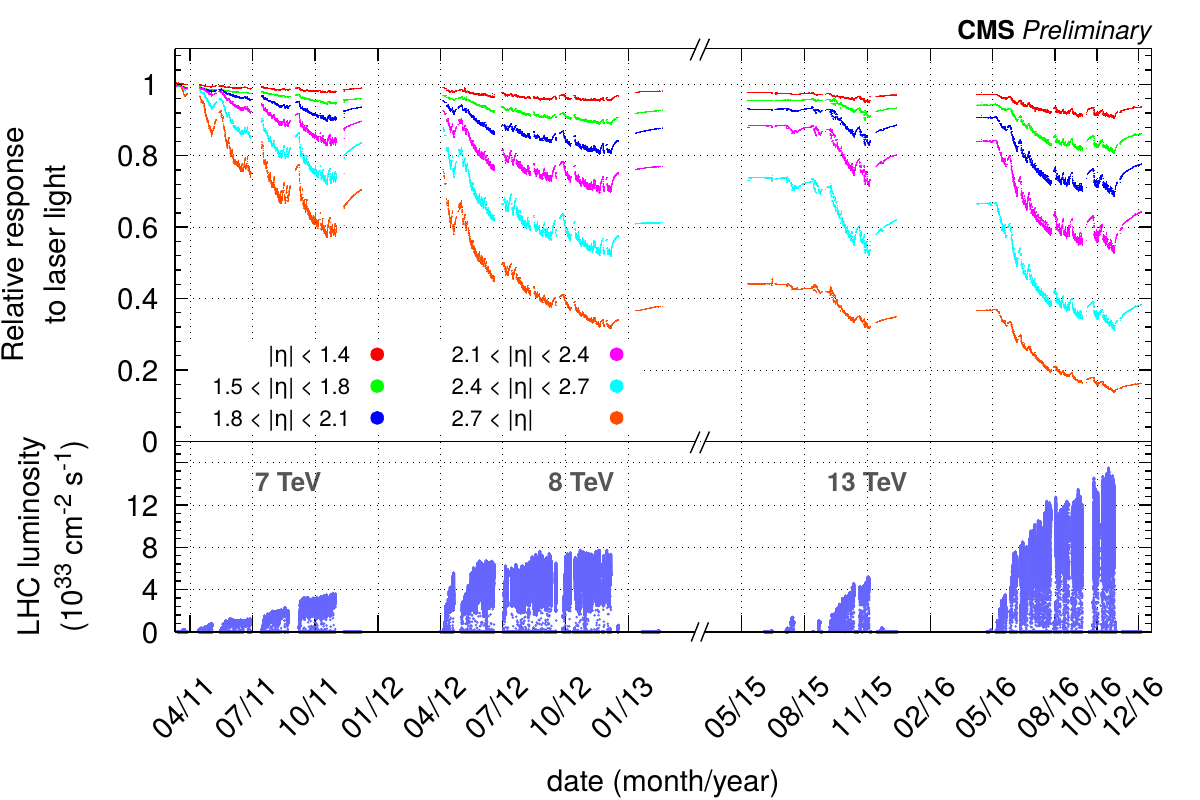
\includegraphics[width=\linewidth]{Figures/Detector/ecal_response.png}
       \caption{ Relative response of the ECAL crystals for the 2011 to 2016 data-taking periods.
       The average observed change in response is up to 10\% in the barrel and 50\% for $|\eta| <$ 2.5. 
       The bottom plot shows the instantaneous luminosity delivered during this period. The crystals recovered 
       some, but not all, of their response during Long Shutdown 1 (2013-2014). Reprinted from Reference~\cite{ECALDPGtwiki}.}
   	\label{fig:ecal_response}
\end{figure*}


The downside to PbWO$_4$ is that it has a relatively low light yield of only 2 photoelectrons per MeV of incident energy. This makes the electronics used to collect the signal especially important. The crystal itself acts as an optical waveguide, and the scintillation light is internally reflected until it reaches the photodetectors glued directly onto the rear face of the crystal. Avalanche photodiodes (APD) are used in the barrel, and vacuum phototriodes (VPT) are used in the more radioactive endcap region. Both of these were chosen to be able to operate within the 3.8 T magnetic field, and both increase the gain by a factor of approximately 1000.
The signal then goes to a Multi-Gain Preamplifier (MGPA), which dynamically changes the gain based on the energy of the incident particle. 
Temperature control of the PbWO$_4$ crystals and the attached APDs is crucial to maintaining an excellent resolution. The crystal response and APD gain change by approximately 2.2\% and 2.4\% per $^\circ$C, respectively. 

The last sections of the ECAL system are two pre-shower detectors located in front of the EE. The pre-shower detector is designed to improve the spatial resolution of the ECAL, so that the two photons from $\pi^0\rightarrow\gamma\gamma$ decays can be distinguished. Each pre-shower detector consists of alternating strips of lead and silicon detectors. The lead forces the photons to interact, and the silicon detector measures the electrons and positrons produced in the shower with high granularity. The pre-shower detector achieves a spatial resolution of 2 mm, compared to the 3 cm resolution of the EB and EE. 


%%%%%%%%%%%%%%%%%%%%%%%%%%%%

\section{Hadron calorimeter (HCAL)}
\label{sec:HCAL}
The hadron calorimeter (HCAL) is the next sub-detector after the ECAL. It is a brass sampling calorimeter, with alternating layers of plastic scintillator and brass absorbers. 
Heavy particles such as hadrons interact with the brass layers, and the scintillation light from the nuclear showers is collected with wavelength-shifting optical fibers embedded in the plastic scintillator. The light is then guided to pixelated hybrid photodiodes and electronics that amplify the signal. Figure~\ref{fig:HCAL_layout} shows a longitudinal slice of the full HCAL system. 

%Heavy particles such as hadrons interact with the brass layers, and the energy of the resulting nuclear shower is detected in the plastic scintillators. 
%When a charged particle passes through the scintillator, the scintillation light is collected with wavelength-shifting optical fibers. 

\begin{figure*}[h!]
	\centering
	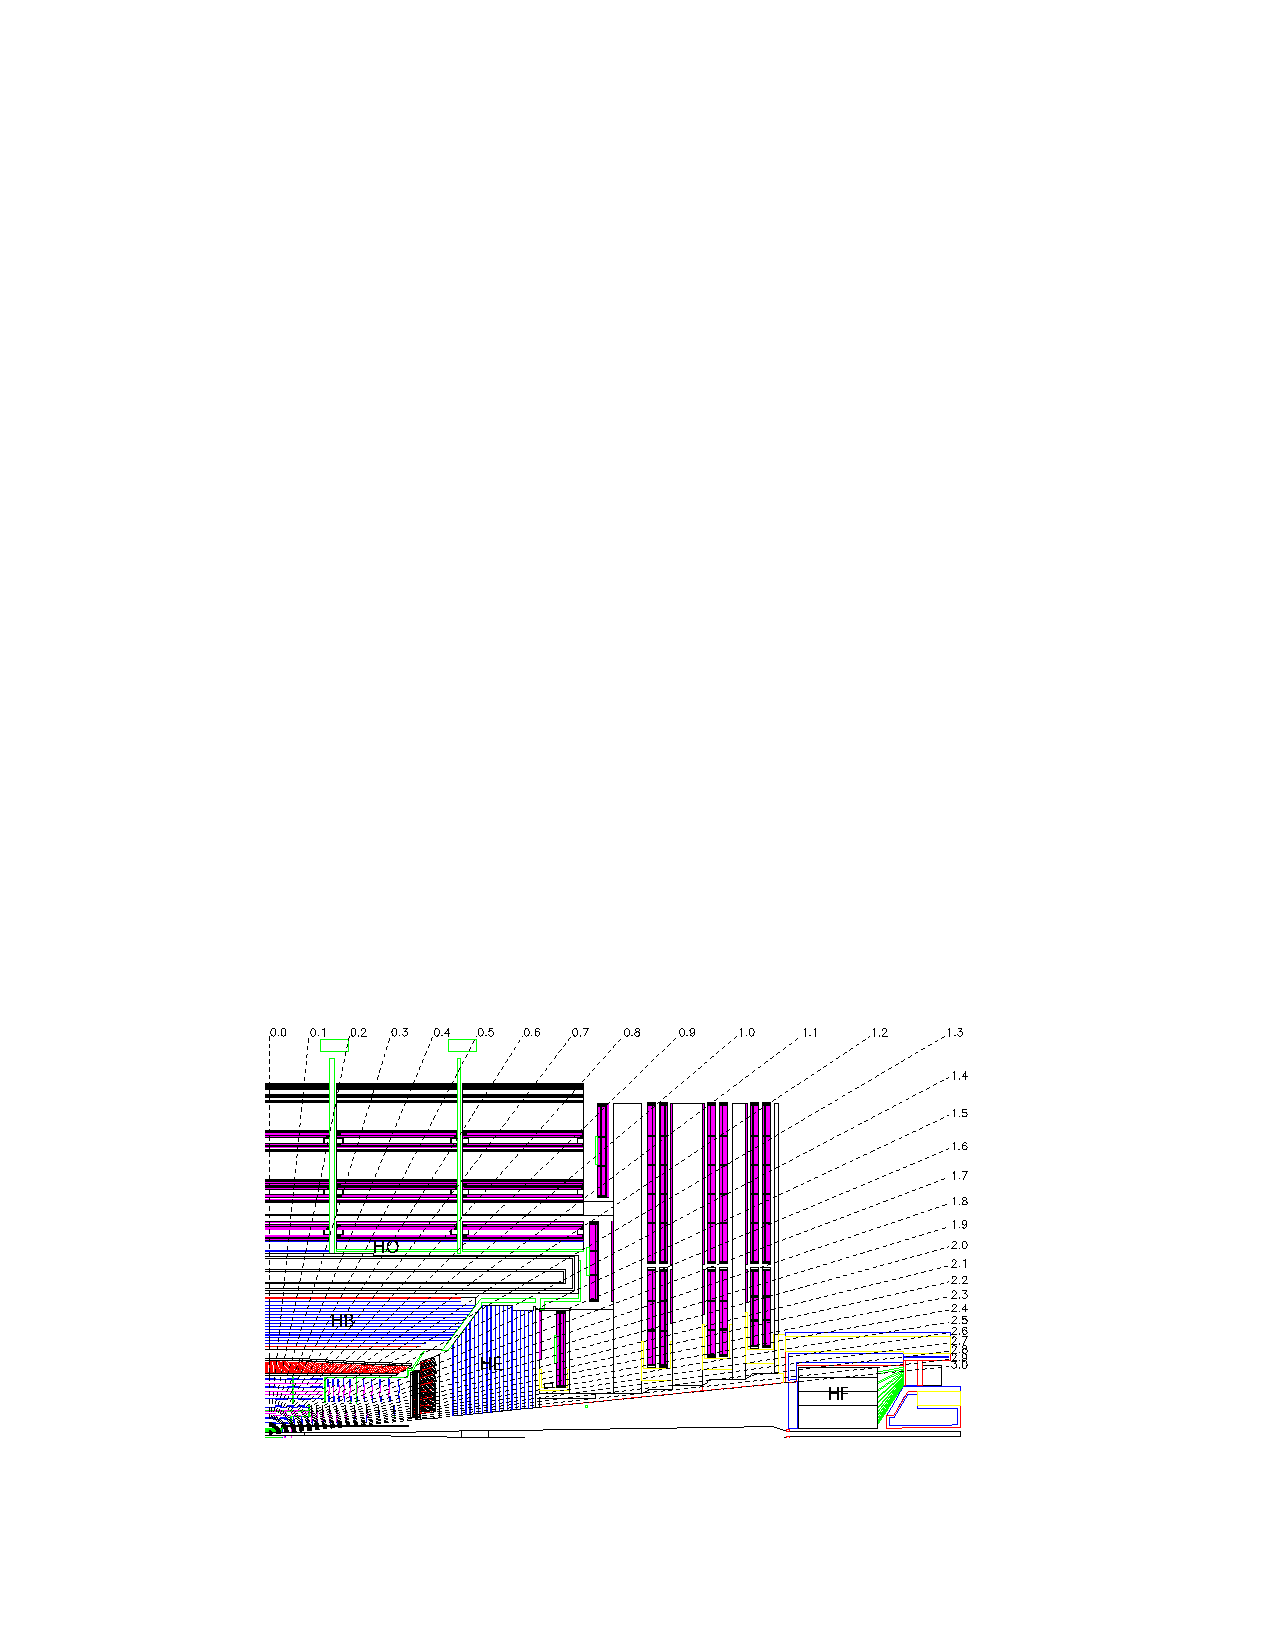
\includegraphics[width=\linewidth]{Figures/Detector/HCAL_layout.pdf}
       \caption{Longitudinal slice of the CMS HCAL, including the barrel HCAL (HB), outer HCAL (HO), endcap HCAL (HE), and forward HCAL (HF). The dashed lines represent lines of constant pseudorapidity. Reprinted from Reference~\cite{Chatrchyan2008zzk}.}
       \label{fig:HCAL_layout}
\end{figure*}

There are 17 scintillator layers in the barrel of the HCAL (HB), which extends radially from 1.77 to 1.95 m and to a pseudorapidity $|\eta| = 1.3$. The first and last layers of absorber are made of steel rather than brass for structural reasons. The scintillation layers are divided into tiles with area $\Delta\phi \times \Delta\eta = 0.87 \times 0.87$. The tiles are further organized into towers that each get a single readout channel. The outer HCAL (HO) is located outside the solenoid and serves to increase the thickness of the calorimeter. 

The HCAL endcap (HE) covers the pseudorapidity range $1.3 < |\eta| < 3$. There are 17 layers of plastic scintillator and 18 layers of absorber in the HE. For $|\eta| < 1.6$, the tile size is the same as those in the barrel, and for $|\eta| >1.6$ the tile size is reduced to $\Delta\phi \times \Delta\eta = 0.17 \times 0.17$. Depending on the pseudorapidity, there are two or three readout channels per tower.
 
The last part of the HCAL system is the forward HCAL (HF) that covers the pseudorapidity range from $3 < |\eta| < 5.2$. Charged particles are detected via Cherenkov radiation in quartz fibers planted in the steel absorber. The quartz fibers were chosen to be able to withstand the high radiation levels of particles emitted close to the beam pipe. 
All three segments of the HCAL are calibrated using radioactive sources $^{136}$Cs or $^{60}$Co mounted on the tip of a moving wire. The radioactive sources produce photons at known energies, allowing for an absolute calibration of each scintillator. 

Because most of the energy from the nuclear showers is deposited in the absorbers rather than the scintillation material, 
the HCAL naturally has a lower energy resolution than the ECAL . In addition, nuclear showers might start 
before particles even reach the HCAL, or charged particles might deposit energy in the ECAL via bremsstrahlung. 
The mean distance traveled by a hadronic particle before undergoing 
an inelastic nuclear interaction is known as the nuclear interaction length. 
The radial depth of the ECAL corresponds to 1.1 nuclear interaction lengths, and
in the HCAL there are 5.82 interaction lengths at $|\eta|=0$ and 10.6 interaction lengths at $|\eta|=1.3$. 
The resolution of the calorimeters is described in more detail below.

At the analysis level, the objects of interest are not individual hadrons, but objects known as jets. A jet is a spray of particles in a narrow cone that is produced by the hadronization of quarks and gluons. The reconstruction of jets is described in detail in Chapter~\ref{sec:EventReconstruction}.

%The relative energy resolution of the two calorimeters together is $\Delta\mathrm{E}/\mathrm{E} \approx 100\% / \sqrt{\mathrm{E}} $. 
%look up energy resolution
%references?
%this is old, but might work https://arxiv.org/pdf/0911.4991.pdf
%conference proceeding http://home.fnal.gov/~chlebana/CMS/PAS/HCALPerformance.pdf


%%%%%%%%%%%%%%%%%%%
\section{Calorimeter performance}
In general, the energy resolution $\sigma/E$ of a calorimeter can be modeled with the following equation where $\oplus$ is used to represent summing in quadrature \cite{Calo}:
\begin{equation}
\frac{\sigma}{E} = \frac{a}{\sqrt{E}} \oplus \frac{b}{E}  \oplus c 
\end{equation}
The first term is a stochastic term that takes into account random fluctuations in the amount of deposited energy for a particle with incident energy $E$. Homogeneous detectors like the ECAL have an excellent intrinsic resolution and a very small stochastic term. Sampling calorimeters such as the HCAL, on the other hand, have larger stochastic terms because the number of charged particles that hit the active layers varies from shower to shower.

The $b/E$ term represents electronic noise from the equipment that is used to collect the signal. This term can depend sensitively on the temperature of the electronics, as already mentioned for the EB APDs. Maximizing the energy yield helps improve this contribution to the energy resolution. The final term is a constant and covers any irregularities in the detector response. This can include variations between ECAL crystals, radiation damage effects, or differences in response due to temperature gradients across the detector.

The resolution of the ECAL as measured using $Z\rightarrow ee$ events in the first 2.5 \fbinv of 13 TeV data is shown in Figure~\ref{fig:ecal_resolution}. For the central region of EB. the electron energy resolution is better than 2\%/E. 
%The energy resolution of objects in the HCAL will be described in more detail in Chapter~\ref{sec:EventReconstruction}.

\begin{figure*}[h!]
	\centering
	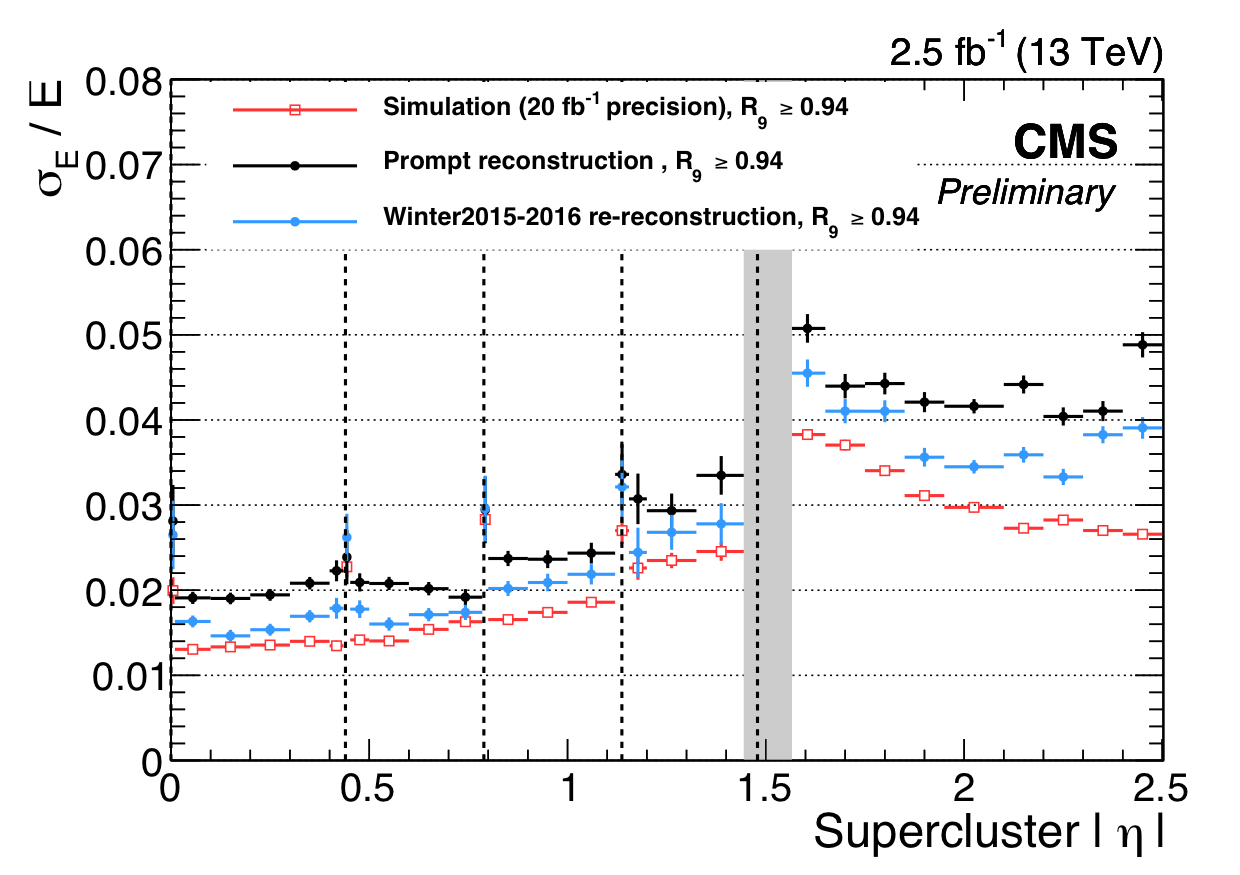
\includegraphics[width=\linewidth]{Figures/Detector/EcalEnergyResolution.png}
       \caption{Relative electron energy resolution in bins of pseudorapidity. 
       The energy resolution was calculated from an unbinned likelihood fit to $Z\rightarrow ee$ events.
        Barrel module boundaries are shown with vertical dashed lines and often correspond to regions where the resolution is somewhat degraded. The gray band at $|\eta|$ = 1.5 represents the boundary between EB and EE.
        The data correspond to 2.5\fbinv collected with the CMS detector in 2015.
        Reprinted from Reference~\cite{ECALDPGtwiki2}.}
         \label{fig:ecal_resolution}
\end{figure*}

The combined energy resolution of the ECAL and HCAL can be expressed as the following \cite{ParticleFlow}:
\begin{equation}
\frac{\sigma}{E} = \frac{110\%}{\sqrt{E}} \oplus 9\% 
\end{equation}
This resolution was measured using a pion test beam. The jet energy resolution after applying the full event reconstruction will be described in more detail in Chapter~\ref{sec:EventReconstruction}.


%%%%%%%%%%%%%%%%%%%%%%%%%%%%

\section{Muon system}
\label{sec:Muon}
Aside from weakly-interacting particles such as neutrinos, muons are the only particles that make it past the HCAL. Muons do not interact via the strong force and are too heavy to be stopped by electromagnetic interactions alone. For this reason, the muon detector system is the outermost layer of CMS. Three different types of detectors are used in the muon system: drift tube (DT) chambers, cathode strip chambers (CSC), and resistive plate chambers (RPC). The muon system is located at a radial distance $r > 3.5$ m and is embedded in the return yoke for the magnetic flux.

A drift tube consists of a conducting wire held at high positive voltage in the center of a gas cell. When a charged particle passes through the gas, the gas is ionized. The freed electrons are drawn to the positively charged wire, and in turn cause more ionization as they are accelerated. The time between the passage of the initial particle and the resulting electron avalanche can be used to reconstruct the position of the interaction perpendicular to the wire.

Drift tubes are used in the barrel region of the detector and extend to $|\eta| < 1.2$. The CMS drift tubes are are made from aluminum plates and contain a mixture of 85\% Ar and 15\% CO$_2$. A gold-plated stainless steel anode wire is located at the center of each tube. The wires are held at 3.6 kV and have a thickness of 50 $\mu$m. Each drift tube has dimensions 1.3 cm $\times$ 4.2 cm $\times$ 2.4 m. Four layers of drift tubes make up a superlayer, and a group of 2 or 3 superlayers makes up one muon chamber.

The endcap system uses cathode strip chambers because of their improved performance in high flux areas and non-uniform magnetic fields. Positively-charged wires are aligned perpendicular to negatively-charged copper strips in a gas, which gets ionized by passing muons. Electrons produce a signal in the anode wires and positive ions produce a signal in the cathode strips. This provides two position coordinates for each muon. The spatial resolution in the azimuthal direction is 150 $\mu$m. The CSCs extend the pseudorapidity coverage of the muon system to $|\eta| < 2.4$.

Finally, resistive plate chambers are used in both the barrel and the endcap for more precise timing measurements. This is important for triggering purposes and to make sure each muon is assigned to the correct bunch crossing. A high voltage is applied to two large plates with a gaseous layer between them. The plates themselves have a high resistance, and the cascade caused by the passage of a muon through the gas is detected via readout strips outside the chamber. The CMS RPCs have a timing resolution of 1 ns. 

%%%%%%%%%%%%%%%%%%%%%%%%%%%%
\section{Instantaneous luminosity measurement}
\label{sec:lumi}

%https://cds.cern.ch/record/2257069?ln=en
Five different detectors (luminometers) are used to measure the instantaneous luminosity $L$ delivered by the LHC \cite{lumiPAS}: the pixel detector, the barrel drift tubes (DT), the forward hadron calorimeter (HF), and two specialized instruments, the Fast Beam Conditions Monitor (BCM1f) and the Pixel Luminosity Telescope (PLT). The last three use a fast readout system that is separate from the rest of the CMS system, and the pixel detector and DT use the standard data acquisition system. 
%cite http://cds.cern.ch/record/2257069/files/LUM-17-001-pas.pdf?version=1

Van der Meer (VdM) scans \cite{VanderMeer} are used to set an absolute calibration of each detector. Dedicated LHC running conditions allow the two beams to be scanned step-wise through one another in the two transverse directions. By finding the optimum beam position in the horizontal and vertical planes, the size of the beams at the collision point can be determined. This in turn is used to calculate the visible cross sections $\sigma_{vis}$ for each detector. The instantaneous luminosity is then given by the following, where $R$ is the measured rate for a given luminometer:
\begin{equation}
L = \frac{R}{\sigma_{vis}}
\end{equation}

The integrated luminosity $\mathcal{L}$ is the integral of all collisions taking place within CMS and represents the total amount of data collected. Figure~\ref{fig:lumi} shows the integrated luminosity delivered to CMS by the LHC and the integrated luminosity recorded by CMS during the 2016 data-taking period for 13 TeV $p$-$p$ collisions. CMS collected 92.5\% of the 40.76 \fbinv delivered by the LHC. CMS can fail to record events delivered by the LHC if any sub-detector is off or if there is trigger deadtime. The 2016 ``golden JSON", the full list of runs and events that are certified for use in data analysis, corresponds to 35.92 \fbinv. The total uncertainty on the integrated luminosity is 2.5\% \cite{lumiPAS}. The LHC is on track to deliver 100 \fbinv over the course of Run II. 

\begin{figure*}[h!]
	\centering
	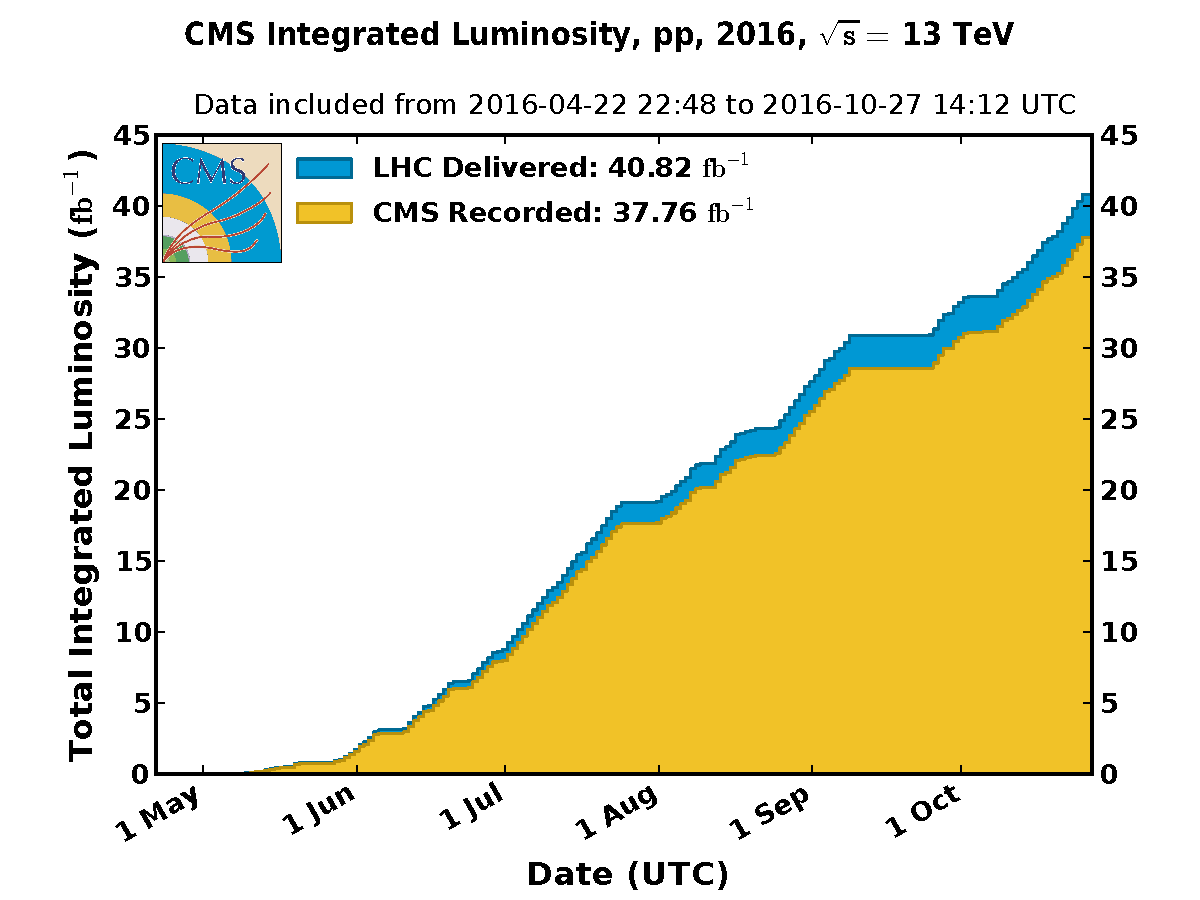
\includegraphics[width=\linewidth]{Figures/Detector/int_lumi_per_day_cumulative_pp_2016.pdf}
       \caption{Integrated luminosity delivered to CMS by the LHC (blue) and the integrated luminosity recorded by CMS (orange) during $p$-$p$ collisions at $\sqrt{s}$ = 13 TeV in 2016.}
         \label{fig:lumi}
\end{figure*}






